\documentclass[../../index.tex]{subfiles}

\begin{document}
\chapter{Measuring the strong coupling}

\section{Fits}
In the following we will perform fits to determine $\alpha_s$ at the
$m_\tau^2$\-/scale. The fits are separated corresponding to the used weight. Every
weight contains multiple fits for different $s_0$\-/momenta. We will start with
the kinematic weight, which appears naturally in the inclusive $\tau$\-/decay
ratio \cref{eq:inclusiveRatio} and has the best fitting characteristics of all
weights we have used.

\subsection{Kinematic weight: $\omega_{\tau}(x) \equiv (1-x)^2(1+2x)$}
The kinematic weight is defined as $\omega(x) = (1-x)^2(1+2x)$. It is a
double pinched, polynomial weight\-/ function that contains the unity and
does not contain a term proportional to x, which makes it an optimal weight
\cite{Beneke2012}. As a doubled pinched weight it should have a good suppression
of \textsc{dv}\-/contributions and its polynomial contains terms proportional to
$x^2$ and $x^3$, which makes it sensitive to the dimension six and eight \textsc{ope}
contributions. The fits have been performed within the framework of \textsc{fopt} for different numbers of $s_0$.
The momentum sets are characterised by its lowest energy $s_{min}$. We
fitted values down to $\SI{1.5}{\giga\eV}$. Going to lower energies is
questionable due to the coupling constant becoming to large, which implies a
breakdown of \textsc{PT} and appearing DVs. Furthermore it bares the
risk to be affected by the $\rho(770)$ and $a_1$ peaks in the vector and
axial-vector spectral function, which we cannot model within the framework of
the \textsc{ope}. For the fitting\-/parameters $\alpha_s, c_6$ and $c_8$ we have given the results in
\cref{table:fitWKinAlD6D8} and graphically in \cref{fig:fitWKinAlD6D8}.
\begin{table}[H]
  \centering
  \begin{tabular}{llllll}
    \toprule \\
    $s_{min}$ & \#$s_0$s & $\alpha_s(m_\tau^2)$ & $c_6$ & $c_8$ & $\chi^2/dof$  \\
    \hline \\
    % 1.500 & 23 & 0.3255(13) & -0.441(10) & -0.2909(34) & 2.00  \\
    % 1.525 & 22 & 0.3255(18) & -0.440(36) & -0.288(45) & 2.10 \\
    % 1.550 & 21 & 0.3265(16) & -0.478(36) & -0.343(50) & 1.81 \\
    % 1.575 & 20 & 0.3269(22) & -0.493(47) & -0.365(58) & 1.86 \\
    % 1.600 & 19 & 0.3272(23) & -0.506(51) & -0.384(64) & 1.94 \\
    % 1.625 & 18 & 0.3284(24) & -0.540(53) & -0.433(68) & 1.788 \\
    % 1.650 & 17 & 0.3283(24) & -0.550(57) & -0.448(74) & 1.90 \\
    % 1.675 & 16 & 0.3284(24) & -0.549(57) & -0.448(79) & 2.04 \\
    % 1.700 & 15 & 0.3281(24) & -0.538(63) & -0.430(87) & 2.19 \\
    % 1.750 & 14 & 0.3291(26) & -0.581(71) & -0.50(10) & 2.21 \\
    % 1.800 & 13 & 0.3293(27) & -0.589(77) & -0.51(11) & 2.43 \\
    % 1.850 & 12 & 0.3281(28) & -0.537(85) & -0.42(13) & 2.5 \\
    % 1.900 & 11 & 0.3272(29) & -0.493(93) & -0.35(15) & 2.65 \\
    1.950 & 10 & 0.3232(32) & -0.31(11) & -0.01(18) & 1.13 \\
    2.000 & 9 & 0.3234(34) & -0.32(12) & -0.03(21) & 1.31 \\
    2.100 & 8 & 0.3256(38) & -0.43(15) & -0.25(28) & 1.30 \\
    \rowcolor{primary}
    2.200 & 7 & 0.3308(44) & -0.72(20) & -0.85(38) & 0.19 \\
    \rowcolor{primary}
    2.300 & 6 & 0.3304(52) & -0.69(25) & -0.80(50) & 0.25 \\
    \rowcolor{primary}
    2.400 & 5 & 0.3339(70) & -0.91(39) & -1.29(83) & 0.10 \\
    2.600 & 4 & 0.3398(15) & -1.3(1.0) & -2.3(2.5) & 0.01  \\
    \bottomrule
  \end{tabular}
  \caption{Table of our fitting values of $\alpha_s(m_\tau^2), c_6$ and $c_8$ for the kinematic weight
    $\omega(x)=(1-x)^2(1+2x)$ using FOPT ordered by increasing $s_{min}$. The
    errors are given in parenthesis after the observed value.}
  \label{table:fitWKinAlD6D8}
\end{table}
\begin{figure}
  \centering
  \includegraphics[width=\textwidth]{./images/fitWKinAlD6D8.eps}
  \caption{Fitting values of $\alpha_s(m_\tau^2), c_6$ and $c_8$ for the kinematic weight
    $\omega(x)=(1-x)^2(1+2x)$ using FOPT for different $s_{min}$. The left graph plots $\alpha_s(m_\tau^2)$ for
    different numbers of used $s_0$s. The right plot contains the dimension six
    and eight contributions to the OPE. Both plots have in grey the $\chi^2$ per
  degree of freedom (dof).}
  \label{fig:fitWKinAlD6D8}
\end{figure}
\begin{figure}
  \centering
  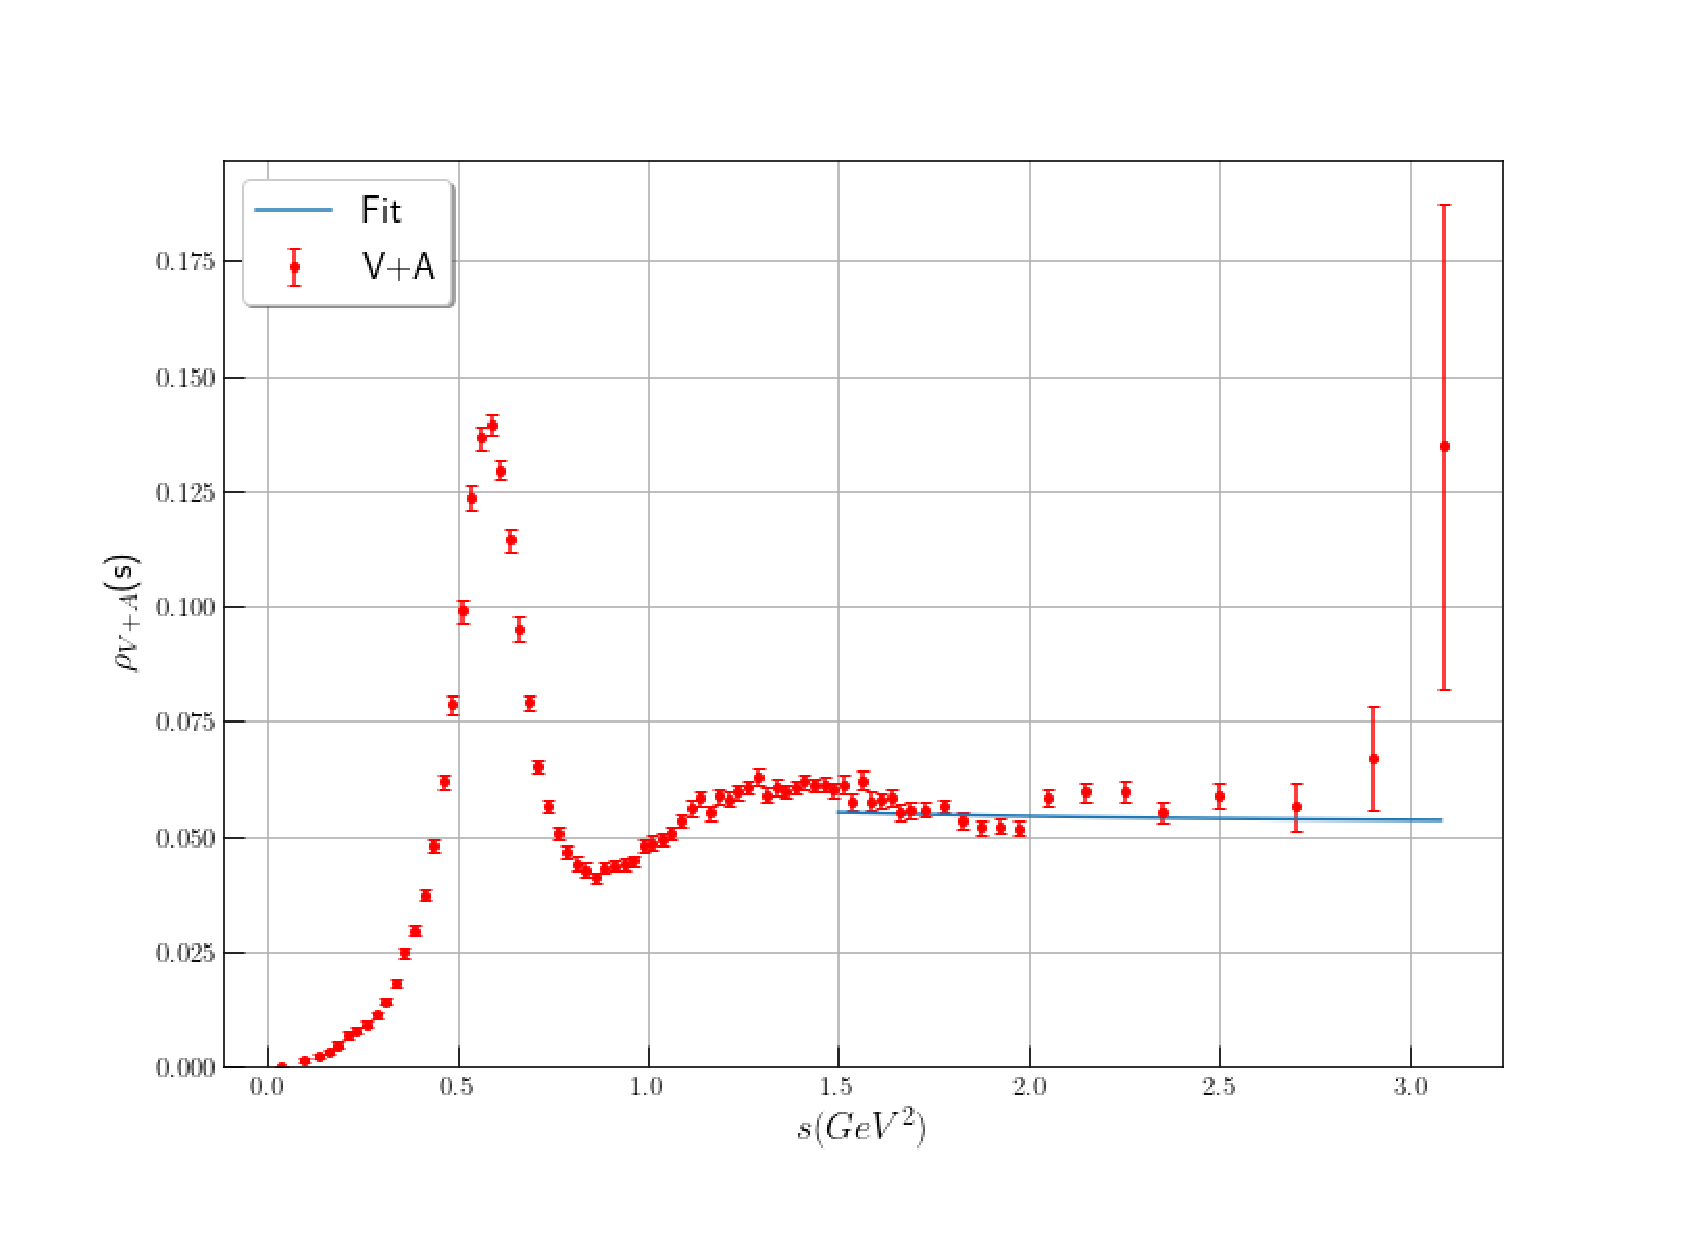
\includegraphics[width=\textwidth]{./images/fitWKinAlD6D8SpecFunc.eps}
  \caption{test}
\end{figure}
We only display the fits for $s_{min}$ larger than \SI{1.95}{\giga\eV} as fits
with higher $s_{min}$ have a too large
$\chi^2$ (larger than two). We achieved six good fits with a $\chi^2$ per \textsc{dof} less or
close to one, which we divided into two groups:
\begin{itemize}
  \item Fits with \textbf{5\-/7} momenta have $\chi^2$ per \textsc{dof} larger
    than one and means of $\alpha(m_\tau^2)=0.3317(33),
    c_6=-0.77(17)$ and $c_8=-0.98(35)$, where we propagated the uncertainty. We
    have excluded the momentum containing four $s_0$s, because it $\chi^2$ is
    too low and its errors are too large, which is because we have to fix three
    variables for only four data points.
  \item Fits with \textbf{8\-/10} momenta have small $\chi^2$ per \textsc{dof}
    values and lower means for the strong
    coupling $\alpha(m_\tau^2)=0.3241(20)$ but the \textsc{ope} contributions
    are higher $c_6=-0.350(75)$ and $c_8=-0.09(12)$.
\end{itemize}
The values for the less momenta are preferred by us due to two reasons. First
below energies of \SI{2.2}{\giga\eV} we have to face the problematic influence
of increasing resonances. Second, we will see, that the values obtained from the
lower moment fits are more compatible with our other fits series. For both, the
momenta sets, we see a good convergence of the \textsc{ope}.

We further tested the stability of the dimension six and eight contributions to
the OPE within the same fit series but for a fixed value of the strong coupling 
to our previous averaged result $\alpha_s(m_\tau^2)=0.3179$. The fits have been
plotted in \cref{fig:fitWKinD6D8} and show good stability. The values for $c_6$
and $c_8$ are larger than the values given in our final results from
\cref{table:fitWKinAlD6D8}. This is explained with a smaller contribution from
the strong coupling ($\alpha_s$ is smaller), which has to be compensated by
larger OPE contributions. 
\begin{figure}
  \centering
  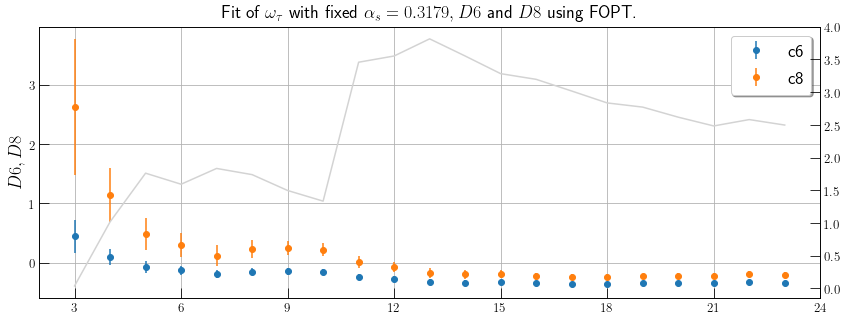
\includegraphics[width=\textwidth]{./images/fitWKinD6D8.eps}
  \caption{}
  \label{fig:fitWKinD6D8}
\end{figure}

Due to the good results we will try to argue in favour of the values obtained by
the lower momenta:
\begin{equation}
  \label{eq:wKinResult}
  \alpha_s(m_\tau^2) = 0.3317(33), \quad c_6 = -0.77(17) \quad \text{and} \quad
  c_8 = -0.98(35).
\end{equation}

\subsection{Cubic weight: $\omega_{cube}(x) \equiv (1-x)^3(1+3x)$}
\label{sec:cubicWeight}
To further consolidate the results from the kinematic weight, we test
a weight of higher pinching, which is known to suppress \textsc{dv} more than a
double pinched weight would do. Consequently, any differences to the previous
fit could indicate a problem with the \textsc{dv} treatment. Our \textit{cubic}
weight will be triple pinched and optimal, as the kinematic weight is double
pinched and we do not want any problematic contributions proportional to $x$.
Thus we define the \textit{cubic weight} as $\omega_{cube}(x) \equiv
(1-x)^3(1+3x)$. It is due to its polynomial structure sensitive to the dimensions
six, eight and ten contributions of the \textsc{OPE}, which yields one more parameter to fit
than with the kinematic weight $\omega_\tau$. The some good, selected fits, by
$\chi^2$ per \textsc{dof}, can be seen in \cref{table:fitWCubicAlD6D8D10} and
graphically in \cref{fig:fitWCubeAlpha}.
\begin{table}
  \centering
  \begin{tabular}{lllllll}
    \toprule \\
    $s_{min}$ & \#$s_0$s & $\alpha_s(m_\tau^2)$ & $c_6$ & $c_8$ & $c_{10}$ & $\chi^2/dof$  \\
    \hline \\
    % 1.800 & 13 & 0.3305(37) & -0.493(76) & -0.48(12) & -0.66(20) & 2.99 \\
    % 1.850 & 12 & 0.3303(37) & -0.482(68) & -0.456(100) & -0.62(17) & 3.35 \\
    1.900 & 11 & 0.3249(29) & -0.280(20) & -0.088(21) & 0.088(55) & 1.58 \\
    1.950 & 10 & 0.3237(26) & -0.232(25) & 0.005(42) & 0.275(93) & 1.67 \\
    2.000 & 9 & 0.3228(26) & -0.196(27) & 0.075(28) & 0.420(56) & 1.96 \\
    \rowcolor{primary}
    2.100 & 8 & 0.3302(40) & -0.52(11) & -0.58(22) & -1.00(45) & 0.43 \\
    \rowcolor{primary}
    2.200 & 7 & 0.3312(43) & -0.56(12) & -0.68(23) & -1.23(50) & 0.55 \\
    \rowcolor{primary}
    2.300 & 6 & 0.336(11) & -0.78(47) & -1.17(98) & -2.38(22) & 0.29 \\
    \rowcolor{primary}
    2.400 & 5 & 0.3330(96) & -0.63(47) & -0.82(10) & -1.51(26) & 0.48 \\
    \bottomrule
  \end{tabular}
  \caption{Table of our fitting values of $\alpha_s(m_\tau^2), c_6$, $c_8$ and
    $c_{10}$ for the cubic weight $\omega(x)=(1-x)^3(1+3x)$ using FOPT ordered
    by increasing $s_{min}$. The errors are given in parenthesis after the observed value.}
  \label{table:fitWCubicAlD6D8D10}
\end{table}
\begin{figure}
  \centering
  \includegraphics[width=\textwidth]{./images/fitWCubeAlD6D8D10.eps}
  \label{fig:fitWCubeAlpha}
\end{figure}
As with the kinematic weight we get two different sets of value:
\begin{itemize}
  \item The fits with \textbf{9, 10 and 11} momenta have a too high $\chi^2$,
    but are comparable to our the upper entries of the kinematic weight table
    \cref{table:fitWKinAlD6D8}. As with the kinematic weight the $s_{min}$ seems
    to be affected by lower resonances.
  \item The fits with \textbf{5,6,7 and 8} have a better $\chi^2$ per
    \textsc{dof} value and are in good agreement with the corresponding fits of
    the kinematic weight. The averaged value with its propagated errors read:
    $\alpha_s(m_\tau^2)=0.332478(61), c_6=-0.622(12), c_8=-0.815(55)$ and $c_{10}=-1.5(3.1)$.
\end{itemize}
We furthermore found that the \textsc{ope} is converging, but not as good as for
the kinematic weight. The values of $\abs{\delta^{(8)}}$ is only half as large
as $\abs{\delta^{(8)}}$.
The values of the lower momentum count are in high agreement with the
ones obtained from the kinematic weight. The
conclusions that we take from the \textit{cubic weight} are that the kinematic
weight, with its double pinching, should sufficiently suppress any contributions
from \textsc{DV}s. If \textsc{DV} would have an effect on the kinematic weight,
we should have seen an improvement of the fits with the \textit{cubic} weight,
due to its triple pinching, which is not the case.

\subsection{Quartic weight: $\omega(x) \equiv (1-x)^4(1+4x)$}
\label{sec:quarticWeight}
To include an even higher pinching of four and to compare the previously
obtained value for the dimension ten \textsc{OPE} contribution we performed fits
with the \textit{quartic weight} defined as $\omega(x) \equiv (1-x)^4(1+4x)$,
which also fulfils the definition of an optimal weight \cite{Beneke2012}. 
Unfortunately the fits only converged for $s_{min}=\SI{2}{\giga\eV}$ (nine $s_0$s
moment combination). The results for , with a $\chi^2$ per \textsc{dof} of $0.67$ are given by:
\begin{equation}
  \begin{split}
  \alpha_s(m_\tau^2) &= 0.3290(11), \quad c_6=-0.3030(46), \quad c_8=-0.1874(28), \\
  c_{10} &= 0.3678(45) \quad \text{and} \quad c_{12}=-0.4071(77)
  \end{split}
\end{equation}
Due to the problematic of the fitting routing, which is caused by too many
\textsc{ope} contributions fitted simultaneously, we will discard the fitting
results for the quartic weight.

\subsection{Third power monomial: $\omega_{m3}(x) \equiv 1-x^3$}
To study the behaviour of the \textsc{DV} and the higher order \textsc{OPE}
contributions of dimension eight and ten we further included two optimal, single pinched weights.
The first one is defined as $\omega_{m3}(x)\equiv 1-x^3$ and contains a
single third power monomial and is consequently sensitive to dimension eight
contributions from the \textsc{OPE}. Our fitting results can be taken from
\cref{table:fitWM3AlD8}.
\begin{table}
  \centering
  \begin{tabular}{lllll}
    \toprule \\
    $s_{min}$ & \#$s_0$s & $\alpha_s(m_\tau^2)$ & $c_8$ &  $\chi^2/dof$  \\
    \hline \\
    % 1.500 & 23 & 0.3160(28) & -0.523(65) & 2.4 \\
    % 1.525 & 22 & 0.3171(28) & -0.578(70) & 2.3 \\
    % 1.550 & 21 & 0.3173(29) & -0.587(76) & 2.42 \\
    % 1.575 & 20 & 0.3187(29) & -0.667(82) & 2.08 \\
    % 1.600 & 19 & 0.3189(30) & -0.679(87) & 2.19 \\
    % 1.625 & 18 & 0.3195(30) & -0.719(94) & 2.24 \\
    % 1.650 & 17 & 0.3205(30) & -0.783(99) & 2.1 \\
    % 1.675 & 16 & 0.3204(31) & -0.77(11) & 2.24 \\
    % 1.700 & 15 & 0.3206(31) & -0.79(11) & 2.39 \\
    % 1.750 & 14 & 0.3202(32) & -0.76(13) & 2.57 \\
    % 1.800 & 13 & 0.3217(33) & -0.88(14) & 2.41 \\
    % 1.850 & 12 & 0.3202(35) & -0.75(16) & 2.4 \\
    % 1.900 & 11 & 0.3202(36) & -0.75(18) & 2.67 \\
    % 1.950 & 10 & 0.3161(38) & -0.40(20) & 1.46 \\
    % 2.000 & 9  & 0.3148(39) & -0.28(22) & 1.47 \\
    % 2.100 & 8  & 0.3147(44) & -0.27(29) & 1.71 \\
    2.200 & 7  & 0.3214(49) & -1.01(39) & 0.41 \\
    2.300 & 6  & 0.3227(57) & -1.18(54) & 0.46 \\
    2.400 & 5  & 0.3257(67) & -1.58(74) & 0.39 \\
    2.600 & 4  & 0.325(10) & -1.54(1.53) & 0.58 \\
    2.800 & 3  & 0.326(21) & -1.69(4.03) & 1.17 \\
    \bottomrule
  \end{tabular}
  \caption{Table of our fitting values of $\alpha_s(m_\tau^2)$, and
    $c_{8}$ for the single pinched third power monomial weight $\omega(x)=1-x^3$ using FOPT ordered
    by increasing $s_{min}$. The errors are given in parenthesis after the observed value.}
  \label{table:fitWM3AlD8}
\end{table}
The $\chi^2$ per \textsc{dof} is like in the $\omega_\tau$ and $\omega_{cubic}$
fits good for $s_{min}\leq \SI{2.2}{\giga\eV}$, but jumps to values
$\chi^2/dof>1.4$ for smaller $s_{min}$. This is, as before, explained through
resonances that appear in lower energies. Due to the good $\chi^2$ and the
internally compatible fitting values we averaged over all rows except the last
one of \cref{table:fitWM3AlD8}. The last row, at $s_{min}=\SI{2.8}{\giga\eV}$
has only one \textsc{dof} and thus high errors. The averaged values are
thus given by 
\begin{equation}
  \alpha(m_\tau^2) = 0.32382(42) \qquad \text{and} \qquad c_8=-1.33(67).
\end{equation}
We note that the strong coupling is smaller as our expected values from the
kinematic weight \cref{eq:wKinResults}, but the dimension eight contribution
is in good agreement. The strong coupling from the monomial weight to third
order seems to be in better agreement with the 8\-/10 momenta used in the
kinematic fits, whereas the dimension eight contributions agrees more with the
4\-/7 momenta fits.

We have made use of a single pinched weight and discovered that the fitting
result is not completely compatible with our previous fitting results.
Consequently weights with a pinching less than two are affected by \textsc{DV}
and should not be used to determine the strong coupling.

\subsection{Fourth power monomial: $\omega_{m4}(x) \equiv
  1-x^4$}
We already analysed the cubic and quartic weights, which depend on the
dimension ten \textsc{ope} contribution, in \cref{sec:cubicWeight}
and \cref{sec:quarticWeight} correspondingly. Now, even with the visible
\textsc{dv} for
fourth power monomial $\omega_{m4}\equiv 1-x^4$ to study another single pinched moment and the dimension
ten \textsc{ope} contribution. The results of the are given in \cref{table:wFitM4AlD10}. 
\begin{table}
  \centering
  \begin{tabular}{lllll}
    \toprule \\
    $s_{min}$ & \#$s_0$s & $\alpha_s(m_\tau^2)$ & $c_{10}$ & $\chi^2/dof$  \\
    \hline \\
    % 1.500 & 23 & 0.3144(27) & -0.572(80) & 2.44 \\
    % 1.525 & 22 & 0.3155(27) & -0.655(90) & 2.34 \\
    % 1.550 & 21 & 0.3157(28) & -0.671(99) & 2.45 \\
    % 1.575 & 20 & 0.3171(28) & -0.80(11) & 2.1 \\
    % 1.600 & 19 & 0.3173(29) & -0.82(12) & 2.21 \\
    % 1.625 & 18 & 0.3180(29) & -0.88(13) & 2.24 \\
    % 1.650 & 17 & 0.3190(30) & -0.98(14) & 2.1 \\
    % 1.675 & 16 & 0.3189(30) & -0.97(15) & 2.24 \\
    % 1.700 & 15 & 0.3192(30) & -1.00(16) & 2.39 \\
    % 1.750 & 14 & 0.3188(32) & -0.96(19) & 2.58 \\
    % 1.800 & 13 & 0.3204(32) & -1.17(21) & 2.39 \\
    % 1.850 & 12 & 0.3190(34) & -0.95(26) & 2.4 \\
    % 1.900 & 11 & 0.3189(35) & -0.94(29) & 2.67 \\
    % 1.950 & 10 & 0.3149(37) & -0.31(34) & 1.47 \\
    % 2.000 & 9  & 0.3137(39) & -0.08(39) & 1.5 \\
    % 2.100 & 8  & 0.3136(43) & -0.07(54) & 1.75 \\
    2.200 & 7  & 0.3203(48) & -1.64(77) & 0.42 \\
    2.300 & 6  & 0.3216(56) & -2.01(1.13) & 0.47 \\
    2.400 & 5  & 0.3247(66) & -2.98(1.62) & 0.39 \\
    2.600 & 4  & 0.324(10) & -2.86(3.69) & 0.58 \\
    2.800 & 3  & 0.325(20) & -3.43(10.74) & 1.17 \\
    \bottomrule
  \end{tabular}
  \caption{Table of our fitting values of $\alpha_s(m_\tau^2)$ and $c_{10}$
    for the single pinched fourth power monomial weight $\omega(x)=1-x^4$ using FOPT ordered
    by increasing $s_{min}$. The errors are given in parenthesis after the observed value.}
  \label{table:fitM4AlD10}
\end{table}
The fitting behaviour is very similar to the third power monomial
(\cref{table:wFitM3AlD8}) and we will directly cite our obtained results:
\begin{equation}
  \alpha_s(m_\tau^2) = 0.32277(40) \qquad \text{and} \qquad c_{10}=-2.4(3.6).
\end{equation}
As before the values for the strong coupling are lower than the ones obtained by
the kinematic weight fit. Furthermore the error on the tenth dimension
contribution of the \textsc{ope} are too huge, although the huge errors makes it
compatible with all previous results. All in all the usage of the single pinched
fourth power monomial weight is questionable and does not deliver any additional insights.

\subsection{Pich's Optimal Moments \cite{Pich2016}}
Next to the previously mentioned \textit{optimal weights} from Beneke and Jamin
\cite{Beneke2012} there are \textit{optimal moments} introduced by Pich
\cite{LeDiberder1992}. Combinations of these optimal moments have been widely
used by the \textsc{aleph} collaboration to perform QCD analysis on the Large electron-positron
collider (\textsc{lep}). These moments include the for \textsc{FOPT} problematic
proportional term in x \cite{Beneke2012}, thus we will perform additional fits
in the Borel-sum.

\begin{equation}
  \omega_{(n,m)}(x) = (1-x)^n\sum_{k=0}^m (k+1)x^k 
\end{equation}
\subsubsection{$\omega(x) = (1-x)^2$}
\begin{table}[H]
  \centering
  \begin{tabular}{llllll}
    \toprule \\
    $s_{min}$ & \#$s_0$s & $\alpha_s(m_\tau^2)$ & $aGGInv$ & $c_{6}$ & $\chi^2/dof$  \\
    \hline \\
    % 1.500 & 23 & 0.3276(13) & -0.0077(10) & 0.330(35) & 2.62 \\
    % 1.525 & 22 & 0.3278(14) & -0.0078(10) & 0.330(38) & 2.75 \\
    % 1.550 & 21 & 0.3299(16) & -0.0092(12) & 0.333(37) & 2.31 \\
    % 1.575 & 20 & 0.3308(25) & -0.0098(13) & 0.334(47) & 2.32 \\
    % 1.600 & 19 & 0.3317(28) & -0.0105(14) & 0.335(54) & 2.38 \\

    % 1.650 & 17 & 0.3345(34) & -0.0124(17) & 0.342(62) & 2.15 \\
    % 1.675 & 16 & 0.3349(25) & -0.0127(15) & 0.342(51) & 2.28 \\
    % 1.700 & 15 & 0.3348(33) & -0.0126(18) & 0.342(58) & 2.47 \\
    % 1.750 & 14 & 0.3372(43) & -0.0145(23) & 0.341(71) & 2.34 \\
    % 1.800 & 13 & 0.3378(31) & -0.0149(20) & 0.339(58) & 2.54 \\
    % 1.850 & 12 & 0.3365(38) & -0.0138(25) & 0.346(60) & 2.72 \\
    % 1.900 & 11 & 0.3355(40) & -0.0128(28) & 0.354(59) & 2.97 \\
    % 1.950 & 10 & 0.3296(47) & -0.0073(34) & 0.418(58) & 1.57 \\
    % 2.000 & 9  & 0.3299(50) & -0.0076(39) & 0.414(64) & 1.83 \\
    % 2.100 & 8  & 0.3331(54) & -0.0108(45) & 0.361(76) & 1.9 \\
    2.200 & 7  & 0.3401(57) & -0.0185(52) & 0.220(88) & 0.73 \\
    2.300 & 6  & 0.3383(68) & -0.0165(67) & 0.26(12) & 0.89 \\
    2.400 & 5  & 0.3450(93) & -0.0243(99) & 0.10(17) & 0.71 \\
    2.600 & 4  & 0.337(16) & -0.014(18) & 0.36(45) & 0.98 \\
    \bottomrule
  \end{tabular}
  \caption{Table of our fitting values of $\alpha_s(m_\tau^2), aGGInv$ and $c_{6}$
    for the triple pinched optimal weight $\omega^{(2,0)}(x)=(1-x)^2$ using FOPT ordered
    by increasing $s_{min}$. The errors are given in parenthesis after the observed value.}
  \label{table:fitOpt30AlD4D6}
\end{table}

\subsubsection{$\omega(x) = (1-x)^3$}
\begin{table}[H]
  \centering
  \begin{tabular}{lllllll}
    \toprule \\
    $s_{min}$ & \#$s_0$s & $\alpha_s(m_\tau^2)$ & $aGGInv$ & $c_{6}$ & $c_{8}$ & $\chi^2/dof$  \\
    \hline \\
    1.900 & 11 & 0.34281(92) & -0.01473(73) & -0.103(22) & -0.534(46) & 1.52 \\
    1.950 & 10 & 0.34154(99) & -0.01304(61) & -0.050(17) & -0.389(44) & 1.42 \\
    2.000 & 9  & 0.33985(81) & -0.01124(43) & 0.002(10) & -0.242(26) & 1.59 \\
    2.100 & 8  & 0.3480(47) & -0.0201(36) & -0.264(89) & -1.03(28) & 0.31 \\
    2.200 & 7  & 0.3483(23) & -0.0204(41) & -0.27(15) & -1.05(40) & 0.41 \\
    2.300 & 6  & 0.3522(64) & -0.0249(62) & -0.42(18) & -1.51(57) & 0.29 \\
    2.400 & 5  & 0.3480(89) & -0.0199(100) & -0.25(33) & -0.96(10) & 0.39 \\
    \bottomrule
  \end{tabular}
  \caption{Table of our fitting values of $\alpha_s(m_\tau^2), aGGInv, c_6$ and $c_{8}$
    for the optimal weight $\omega^{(3,0)}(x)=(1-x)^3$ using FOPT ordered
    by increasing $s_{min}$. The errors are given in parenthesis after the observed value.}
  \label{table:fitOpt30AlD4D6D8}
\end{table}

\newpage
\subsection{Comparison}
To create an overview of our previous results we have gathered the most
compatible rows by hand. These are shown in \cref{table:fitCombinations}, which
is composed of two parts:
\begin{itemize}
\item The upper three rows represent fits we found to have good properties for
  determining the strong coupling.
\item The lower five rows are problematic fits due to too many OPE
  contributions, too low pinching or to terms proportional to $x$.
\end{itemize}
\begin{table}
  \centering \resizebox{\textwidth}{!}{
    \begin{tabular}{cccccccc}
      \toprule \\
      weight & $s_{min}$ & $\alpha_s(m_\tau^2)$ & $aGGInv$ & $c_6$ & $c_8$ & $c_{10}$ & $\chi^2/dof$  \\
      \toprule \\
      $\omega_{kin}$ & 2.2 & 0.3308(44) & - & -0.72(20) & -0.85(38) & - & 0.19 \\
      $\omega_{cube}$ & 2.1 & 0.3302(40) & - & -0.52(11) & -0.58(22) & -1.00(45) & 0.43 \\ 
      $\omega_{3,0}^*$ & 2.1 & 0.3239(30) & -0.2125(26) & -0.627(87) & -0.74(17) & - & 0.46 \\
      \hline \\
      $\omega_{quartic}$ & 2.0 & 0.3290(11) & - & -0.3030(46) & -0.1874(28) & 0.3678(45) & 0.67 \\
      $\omega_{m3}$ & 2.2 & 0.3214(49) & - & - & -1.01(39) & - & 0.41 \\
      $\omega_{m4}$ & 2.2 & 0.3203(48) & - & - & - & -1.64(77) & 0.42 \\
      $\omega_{2,0}$ & 2.2 & 0.3401(57) & -0.0185(52) & 0.220(88) & - & - & 0.73\\
      $\omega_{3,0}$ & 2.1 & 0.3480(47) & -0.0201(36) & -0.264(89) & -1.03(28) & - & 0.31\\
      \bottomrule
    \end{tabular}
  }
  \caption{Table of the best fits (selected by $\chi^2/dof$ and compatibility of
    the fitting values) for each weight including at least the strong coupling
    $\alpha_s(m_\tau^2)$ as a fitting variable. All fits have been performed
    using \textsc{fopt}, except weights marked with a star $\omega^*$, which
    have been fitted using the \textit{Borel sum}.}
  \label{table:fitCombinations}
\end{table}
We have found that the kinematic weight is in excellent agreement with the cubic
$\omega_{cube}$ and Pich's optimal weight $\omega_{3,0}$, fitted using the borel
model. The fitted parameters from the kinematic weight ($\alpha_s, c_6$ and
$c_8$) are all within error ranges and thus compatible. One fact that has to be
investigated is the negative appearing sign for the gluon\-/condensate from the
borel\-/sum of $\omega_{3,0}$.

% \begin{figure}[H]
%   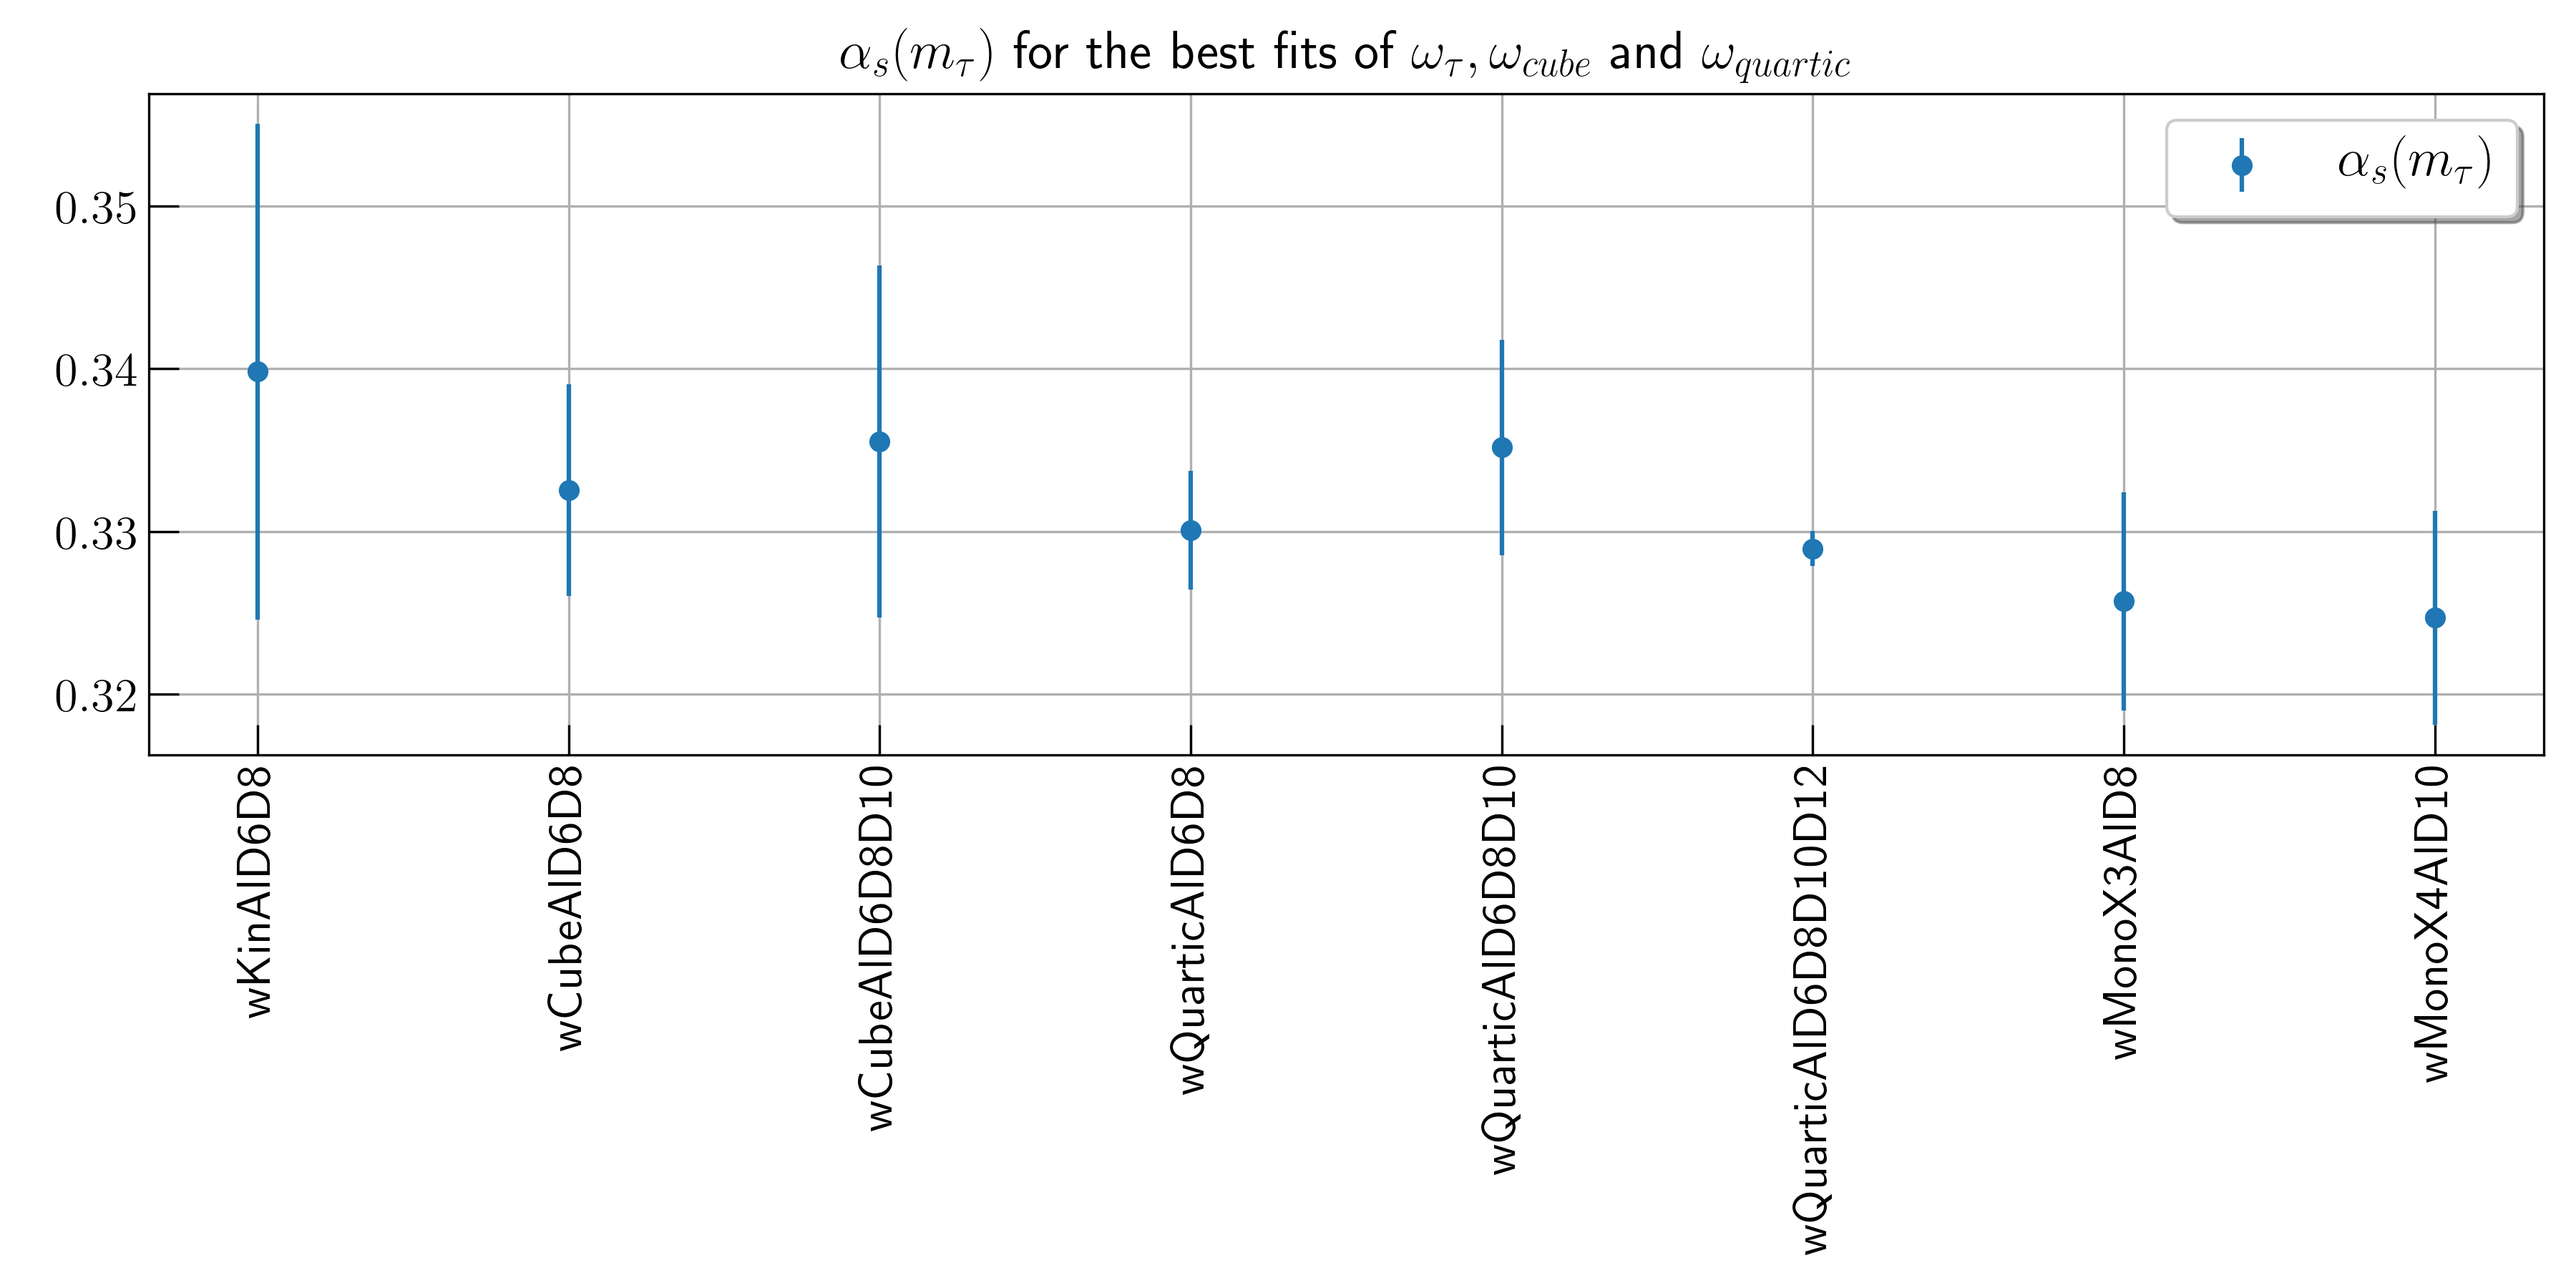
\includegraphics[width=\textwidth]{./images/comparisonAlpha.png}
%   \caption{Comparison of the strong coupling for the best fits (selected by
%   $\chi^2/dof$ closest to one) for each weight including the strong coupling
%   as a fitting variable.}
% \end{figure}
% \begin{figure}[H]
%   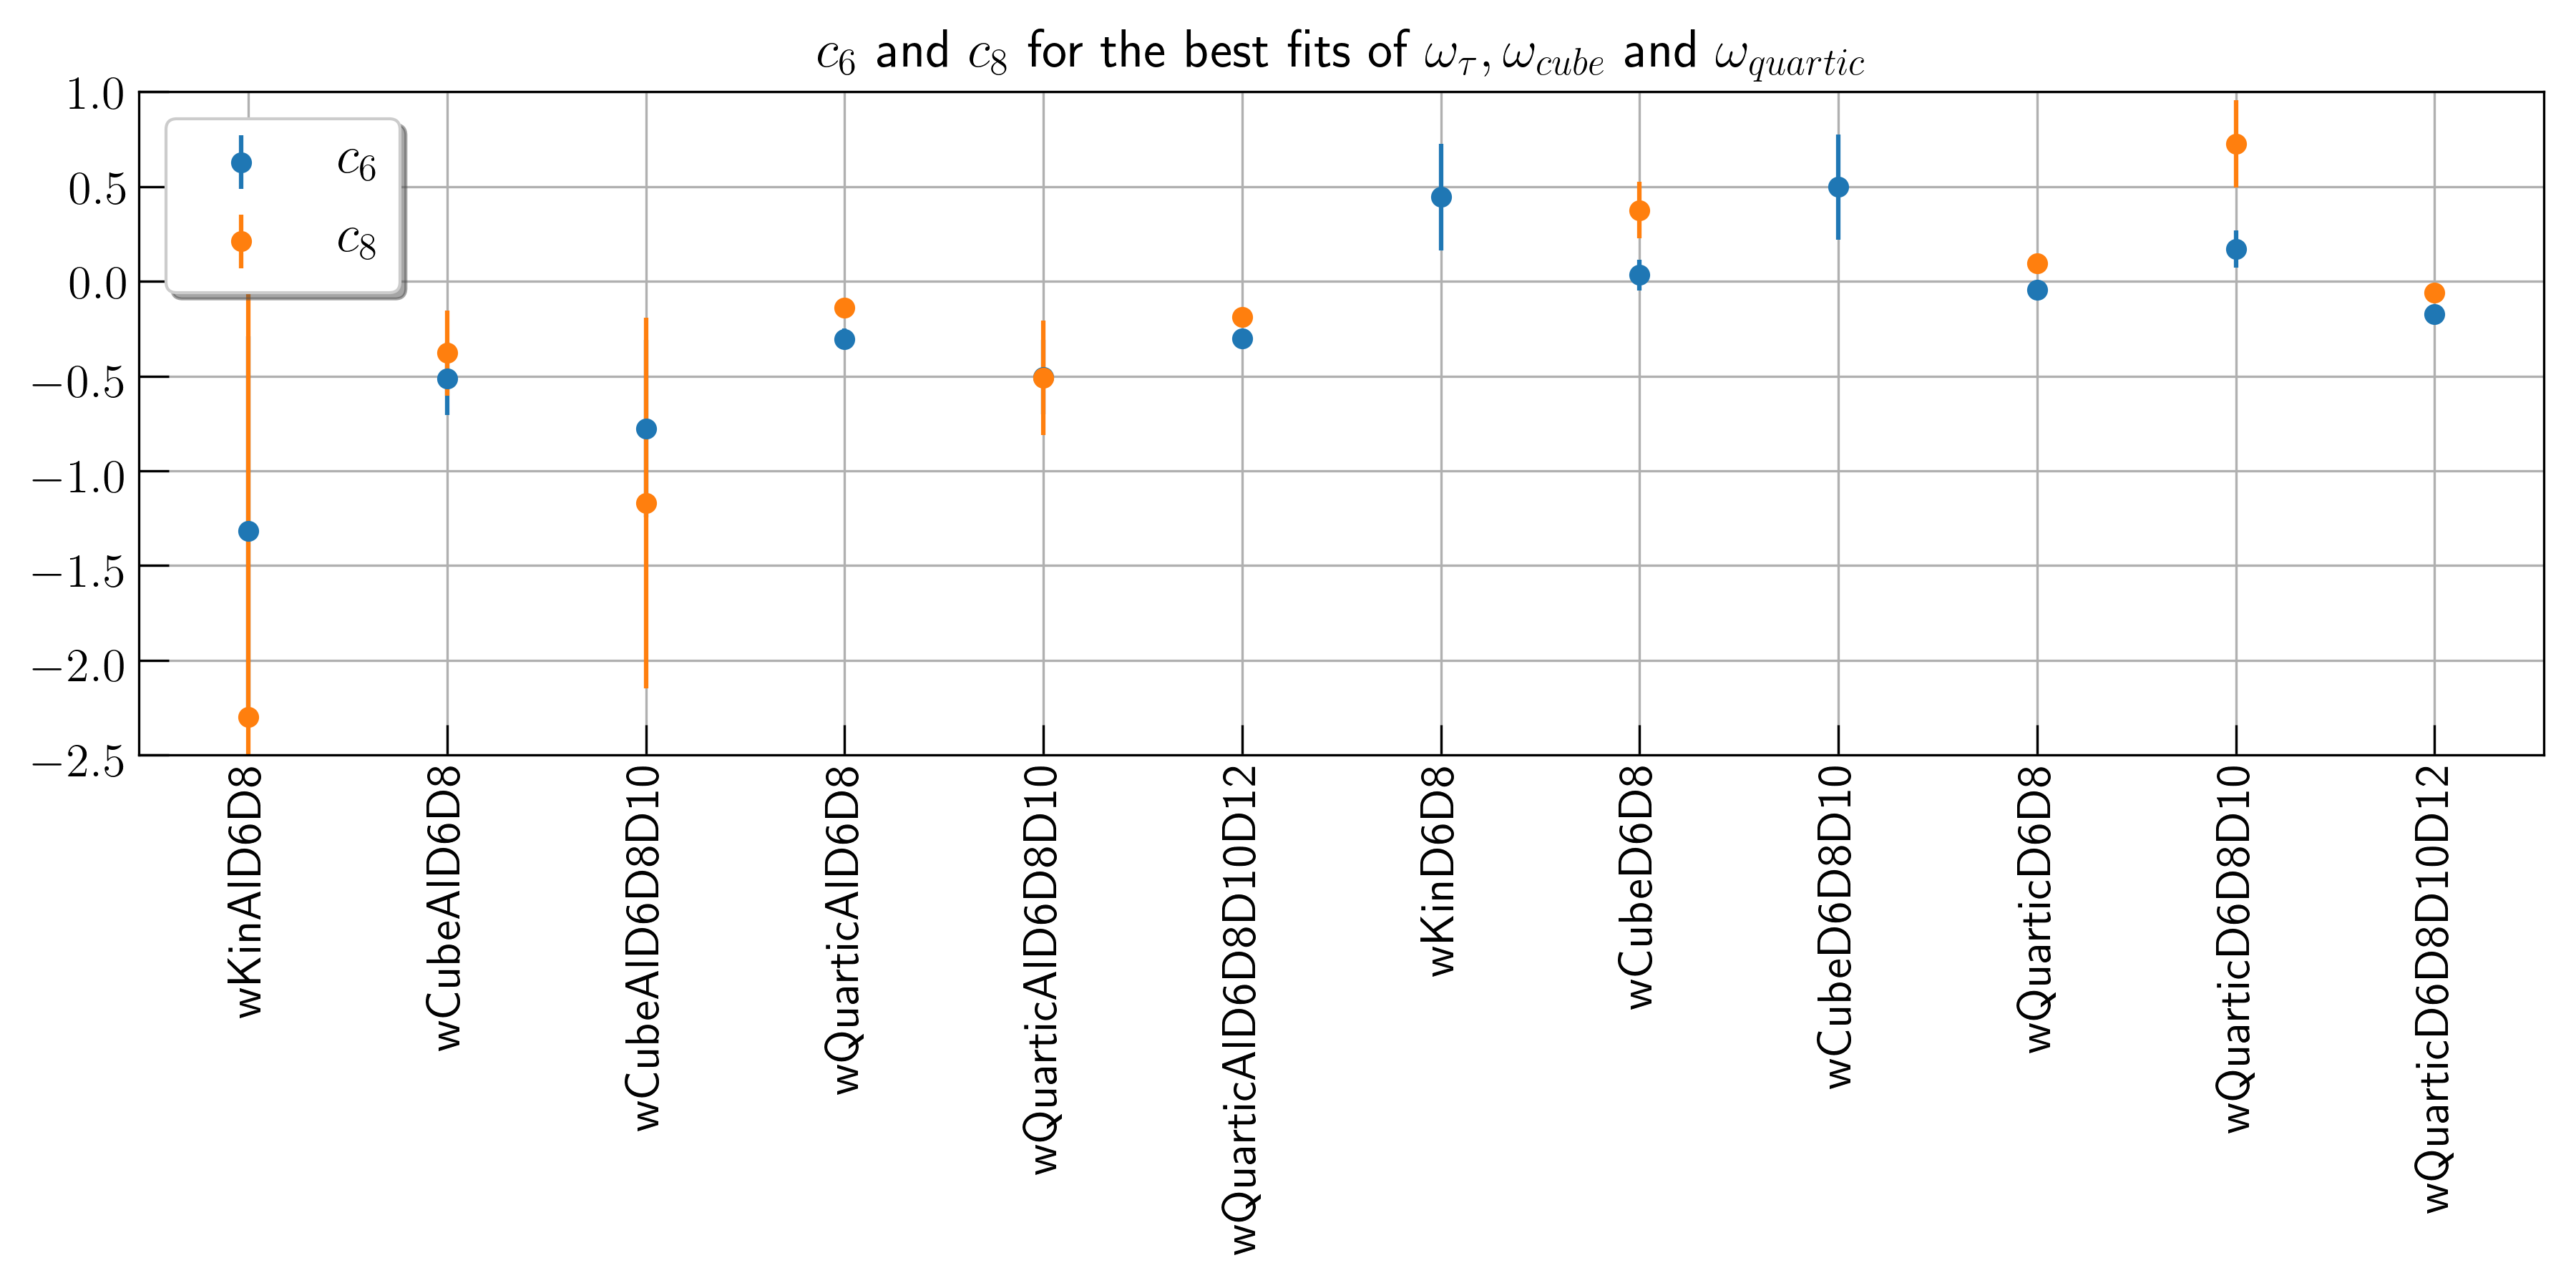
\includegraphics[width=\textwidth]{./images/comparisonD6D8.png}
%   \caption{Comparison of the dimension six and eight values for the best fits
%   (selected by $\chi^2/dof$ closest to one) for each weight including the OPE
%   dimensions six and eight as fitting variables.}
% \end{figure}
% \begin{figure}[H]
%   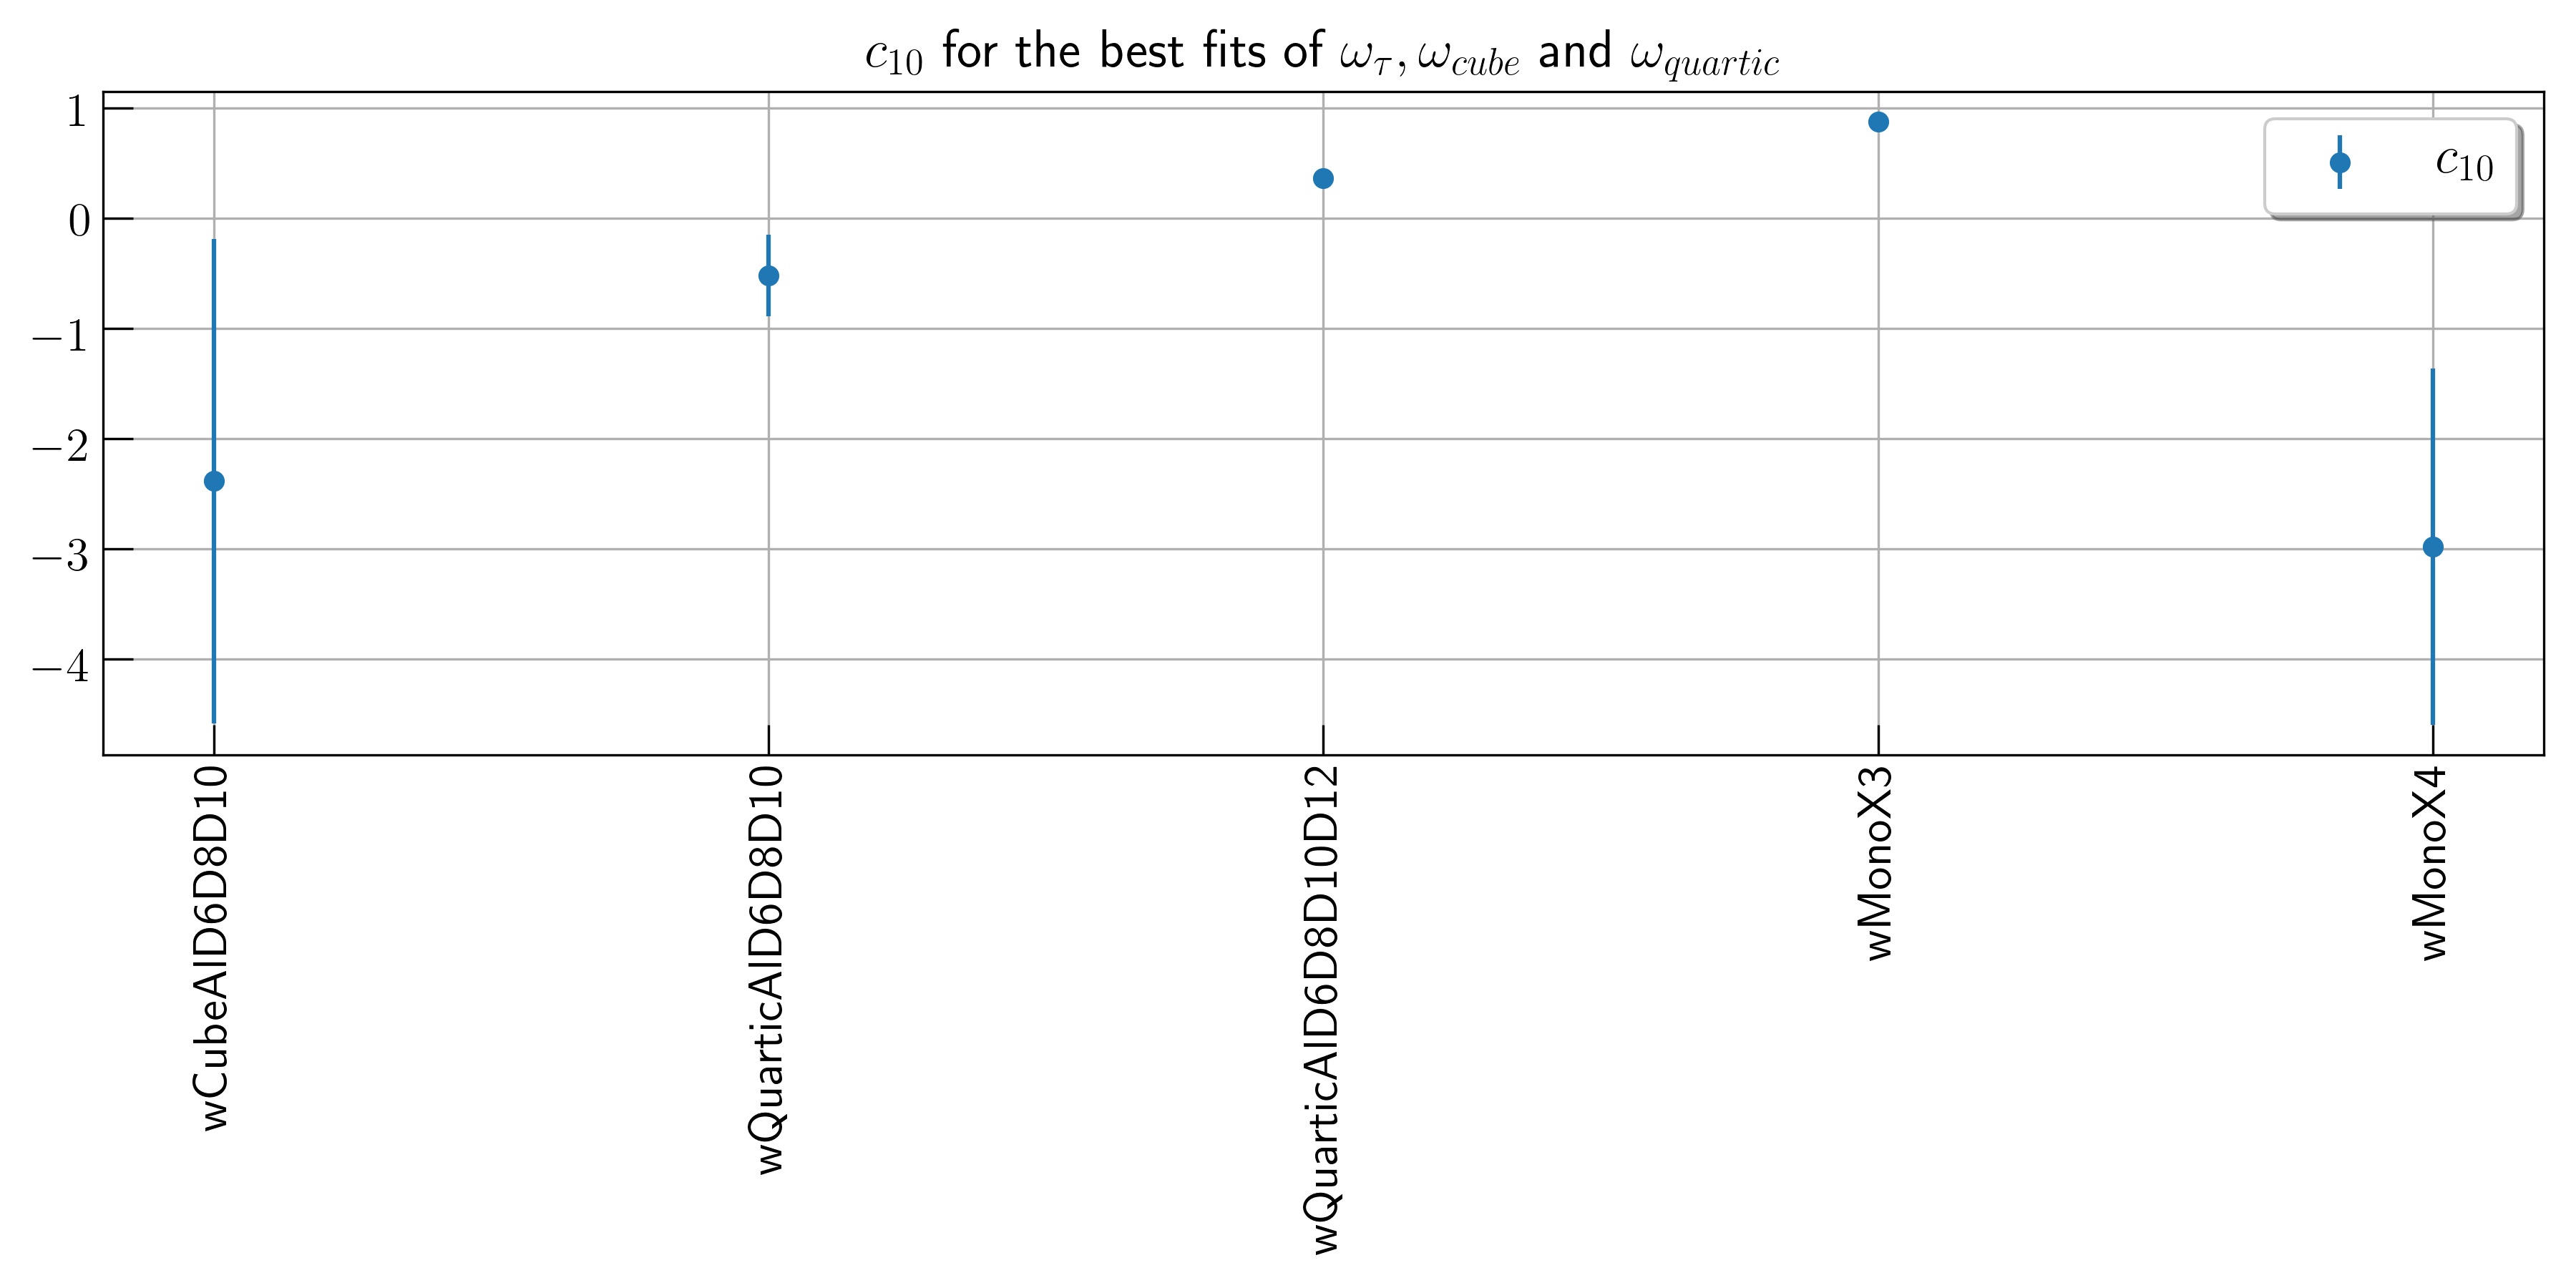
\includegraphics[width=\textwidth]{./images/comparisonD10.png}
%   \caption{Comparison of the dimension ten values for the best fits (selected
%   by $\chi^2/dof$ closest to one) for each weight including the OPE dimensions
%   ten as fitting variables.}
% \end{figure}


\newpage
\subsection{Toni Pich 2006}
\subsubsection{4. ALEPH determination}
Toni built moments with five different weights:
\begin{equation}
  \omega_{kl(x)} = ( 1 - x )^{2+k} x^l (1+x) \quad \text{with} \quad (k,l) = {(0,0), (1,0), (1,1), (1,2), (1,3)}
\end{equation}
He always fitted weight combinations, which we do not include.

\subsubsection{5. Optimal moments}
Used single moments 
\begin{equation}
  \omega^{(n,m)}(x) = (1-x)^n\sum_{k=0}^n (k+1)x^k \quad \text{with} \quad (n,m) = {(1,0), (1,1), (1,2), (1,3), (1,4), (1,5), (2,0), (2,1), (2,2), (2,3), (2,4), (2,5)}
\end{equation}
but omitted NPT corrections! He fitted the kinematic weight with free $\alpha_s$
for $\omega(x)^{(2,1)}$. Later on he uses combined fits which is not in our interest.
It is called optimal moments, because $n$ stands for the pinching factor, which
suppresses DV!

\subsubsection{6. Including information from the $s_0$ dependence}
Pich fits $A^{(2,0)}, A^{(2,1)}$ and $A^{(2,2)}$ separately for $s_{min}=\SI{2}{\giga\eV}$.
The corresponding weights with fitted OPE dimensions are given by:
\begin{align}
  \omega^{(2,0)} &= (1-x)^2 \quad c_4, c_6 \\
  \omega^{(2,1)} &= \omega_{\tau} \quad c_6, c_8 \\
  \omega^{(2,2)} &= (1-x)^2(1+2x+x^2) = (x^2-1)^2 \quad c_8, c_{10}
\end{align}
Thus we can compare our results from the kinematic weight with his results and
furthermore add $(1-x)^2$ to our fitting list?

Alpha is comparable, which just have a bigger error. For D6 and D8 we have to
compare our definition of $c_6, c_8$ with his.

\end{document}